\section{The MuGuard-Flake Framework}
\label{sec:methodology}

\textsc{MuGuard-Flake} embeds a fail-closed local mutation gate inside an iterative repair loop built for pull-request CI (Figure~\ref{fig:architecture}). Two properties keep online overhead practical. First, production code $P_0$ remains fixed, so baseline obligations $M_{\text{det}}(T_{\text{orig}})$ and any partner baseline $M_{\text{det}}(T_{\text{part}})$ are pre-computed once offline. Second, candidate patches reach mutation probing only after passing compilation and stability reruns ($W^+$).

\begin{figure*}[t]
\centering
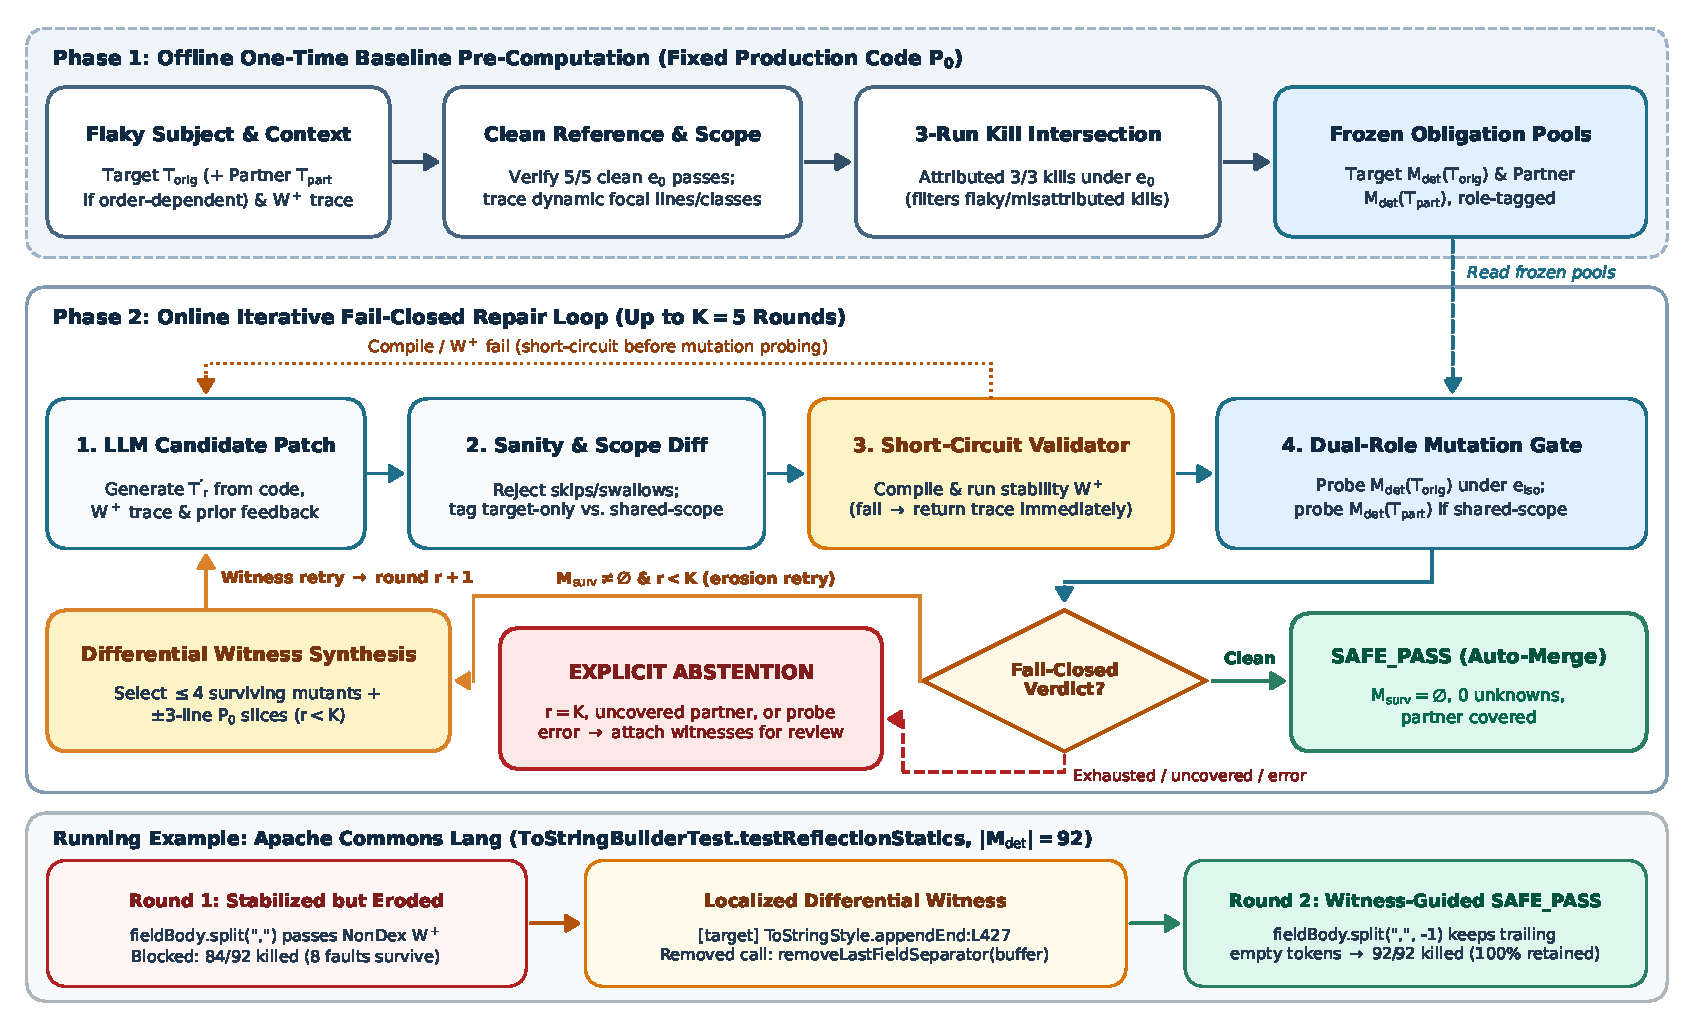
\includegraphics[width=0.93\textwidth]{figures/fig0_muguard_architecture.pdf}
\caption{End-to-end architecture of \textsc{MuGuard-Flake}, showing offline one-time baseline pre-computation, the online fail-closed iterative repair loop, and the two-round \texttt{ToStringBuilderTest} running example.}
\label{fig:architecture}
\end{figure*}

\subsection{Four-Component Fail-Closed Repair Architecture}

\textsc{MuGuard-Flake} pairs offline baseline construction with up to $K = 5$ iterative repair rounds (Algorithm~\ref{alg:muguard}). Given $T_{\text{orig}}$, its $W^+$ failure trace, and surrounding class context (including $T_{\text{part}}$ when order-dependent), each round executes four stages:

\paragraph{Component 1: Single-Test Baseline Pre-Computation.}
Before repair begins, \textsc{MuGuard-Flake} verifies five clean-$e_0$ passes, traces dynamically covered focal scope, and computes the three-run attributed obligation baseline $M_{\text{det}}(T_{\text{orig}})$ from Section~\ref{sec:construct}. Both language backends isolate execution strictly to the target method rather than running whole test classes. For order-dependent tests, partner obligations $M_{\text{det}}(T_{\text{part}})$ are pre-computed independently under the same protocol.

\paragraph{Component 2: Affected-Scope Diff Analysis and Short-Circuit Validator.}
In round $r$, \textsc{MuGuard-Flake} rejects malformed patches (empty bodies, skip markers, or bare exception swallowing) and diffs the target test, partner, and build files, ignoring formatting noise and preserving semantic literals. Edits confined to the target test are tagged \emph{target-only}. Edits touching the partner method, class fields, setup or teardown fixtures, shared helpers, shadowed imports, or build dependencies are tagged \emph{shared-scope} for dual-role gating. The short-circuit validator then compiles candidate $T'_r$ and executes $W^+$. Any compile or stability failure short-circuits immediately and returns diagnostics for the next round without invoking mutation probing.

\paragraph{Component 3: Fail-Closed Dual-Role Conservation Gate.}
Once $T'_r$ passes $W^+$, \textsc{MuGuard-Flake} probes $M_{\text{det}}(T_{\text{orig}})$ under isolated execution $e_{\text{iso}}$ and, for shared-scope order-dependent edits, probes $M_{\text{det}}(T_{\text{part}})$. Two fail-closed invariants govern probing:
\begin{enumerate}[nosep]
    \item \emph{Uncovered-partner closure.} If an order-dependent edit affects shared scope with $|M_{\text{det}}(T_{\text{part}})| = 0$, partner erosion cannot be verified. The gate never accepts the patch, requesting a target-local rewrite on retry or abstaining at round $K$.
    \item \emph{Probe-failure closure.} Any target or partner probe error, timeout, or indeterminate mutant status triggers a retry or abstention rather than silent acceptance or mislabeling as erosion.
\end{enumerate}
Only a clean probe with an empty role-tagged surviving set ($M_{\text{surv}}(T'_r) = \emptyset$) earns a safe pass.

\paragraph{Component 4: Differential Witness Synthesis and Explicit Abstention.}
If $T'_r$ stabilizes with surviving obligations before round $K$, \textsc{MuGuard-Flake} selects up to four role-tagged surviving mutants $m^* \in M_{\text{surv}}(T'_r)$ and synthesizes a localized differential witness:
\begin{equation}
\label{eq:witness}
\begin{aligned}
\omega(m^*) = \big\langle & \text{Role}(m^*),\; \text{Class/File}(m^*),\; \text{Method}(m^*), \\
                          & \text{Line}(m^*),\; \text{OpDesc}(m^*),\; \text{FocalSlice}(P_0, m^*, \pm 3\text{ lines}) \big\rangle.
\end{aligned}
\end{equation}
Following Salva's error-control framing~\cite{salva2026nltestrunner}, if all $K$ rounds end without a clean pass, \textsc{MuGuard-Flake} abstains explicitly rather than merging a degraded test. It records the terminal cause and attaches the surviving-mutant witnesses or failure traces to the pull request, giving human reviewers or hybrid triage assistants concrete production counterexamples to separate valid canonicalization from genuine oracle weakening.

\paragraph{Running Example: Witness-Guided Recovery on \texttt{ToStringBuilderTest}.}
Figure~\ref{fig:architecture} (bottom) traces our Apache Commons Lang running example, \texttt{testReflectionStatics} in \texttt{ToStringBuilderTest} ($|M_{\text{det}}| = 92$). In Round~1, the LLM removes reflection-order flakiness by splitting the serialized field body with single-argument \texttt{split(",")} and sorting the parts. That draft compiles and passes all five \textsc{NonDex} permutations, so single-sided validators accept it immediately. \textsc{MuGuard-Flake}, however, detects eight surviving obligations in \texttt{ToStringStyle} (84/92 killed) and emits the verbatim witness excerpt in Listing~\ref{lst:witness_example}. Pinpointing the removed call to \texttt{removeLastFieldSeparator} reveals that single-argument \texttt{split(",")} drops trailing empty tokens. On Round~2, the model switches to \texttt{split(",", -1)}, restoring 92/92 obligation kills and earning a safe pass.

\begin{lstlisting}[caption={Verbatim differential witness excerpt for Round~1 of \texttt{ToStringBuilderTest} (\texttt{split(",")}, 84/92 killed), exposing the masked trailing-separator fault and guiding Round~2 to \texttt{split(",", -1)} (92/92 killed).},label={lst:witness_example}]
[target] org.apache.commons.lang3.builder.ToStringStyle::appendEnd (L427)
Mutator: VoidMethodCallMutator -- removed call to ToStringStyle::removeLastFieldSeparator
   L425: public void appendEnd(final StringBuffer buffer, final Object object) {
   L426:     if (!this.fieldSeparatorAtEnd) {
>> L427:         removeLastFieldSeparator(buffer);
   L428:     }
   L429:     appendContentEnd(buffer);
\end{lstlisting}

\begin{algorithm}[t]
\caption{\textsc{MuGuard-Flake}: Fail-Closed Mutation-Preserving Flaky Test Repair Loop}
\label{alg:muguard}
\scriptsize
\begin{algorithmic}[1]
\Require Production code $P_0$, flaky test $T_{\text{orig}}$ (and partner $T_{\text{part}}$ if order-dependent), clean config $e_0$, stability family $W^+$, max rounds $K$
\Ensure Terminal gate verdict $d \in \{\texttt{SAFE\_PASS}, \texttt{ABSTAIN\_*}\}$ and verified patch $T^*$ (or $\bot$)
\State Verify $5/5$ clean-$e_0$ passes of $T_{\text{orig}}$; trace focal scope $\mathcal{C}_{\text{focal}}(T_{\text{orig}})$
\State $M_{\text{det}}(T_{\text{orig}}) \gets 3/3$ attributed kills in $\mathcal{C}_{\text{focal}}(T_{\text{orig}})$ under $e_0$
\State If order-dependent, pre-compute standalone $3/3$ attributed partner obligations $M_{\text{det}}(T_{\text{part}})$
\State $\text{feedback} \gets \emptyset$, $T_{\text{prev}} \gets \bot$
\For{$r = 1$ \textbf{to} $K$}
    \State $T'_r \gets \text{LLMRepair}(T_{\text{orig}}, T_{\text{part}}, \text{ContextHeaders}, W^+_{\text{diag}}, T_{\text{prev}}, \text{feedback})$
    \If{$\neg \text{BasicSanity}(T_{\text{orig}}, T'_r)$}
        \State $\text{feedback} \gets \text{SanityErrors}(T'_r)$; $T_{\text{prev}} \gets T'_r$; \textbf{continue}
    \EndIf
    \State $\text{scope} \gets \text{AnalyzeAffectedFileDiff}(T_{\text{orig}}, T_{\text{part}}, T'_r, \text{build})$
    \If{$\neg \text{Compiles}(P_0, T'_r)$}
        \State $\text{feedback} \gets \text{CompileDiagnostics}(P_0, T'_r)$; $T_{\text{prev}} \gets T'_r$; \textbf{continue}
    \EndIf
    \If{$\neg \text{Passes}(P_0, T'_r, W^+)$} \Comment{Short-circuit prior to focal mutation}
        \State $\text{feedback} \gets \text{StabilityTrace}(P_0, T'_r, W^+)$; $T_{\text{prev}} \gets T'_r$; \textbf{continue}
    \EndIf
    \If{order-dependent $\land$ $\text{scope} = \texttt{SHARED\_SCOPE}$ $\land$ $|M_{\text{det}}(T_{\text{part}})| = 0$}
        \State \textbf{if} $r < K$ \textbf{then} $\text{feedback} \gets \text{RequestTargetLocalIsolation}()$; $T_{\text{prev}} \gets T'_r$; \textbf{continue}
        \State \textbf{else} \Return $(\texttt{ABSTAIN\_PARTNER\_UNCOVERED}, \bot)$ \Comment{Fail-closed: never accept}
    \EndIf
    \State $(ok_t, S_t) \gets \text{ProbeFocalMutants}(P_0, T'_r, M_{\text{det}}(T_{\text{orig}}), e_{\text{iso}})$
    \State $(ok_p, S_p) \gets \text{ProbePartnerIfAffected}(P_0, T'_r, T_{\text{part}}, M_{\text{det}}(T_{\text{part}}), \text{scope})$
    \If{$\neg ok_t \lor \neg ok_p$}
        \State \textbf{if} $r < K$ \textbf{then} $\text{feedback} \gets \text{ProbeErrorDiag}()$; $T_{\text{prev}} \gets T'_r$; \textbf{continue}
        \State \textbf{else} \Return $(\texttt{ABSTAIN\_EVAL\_ERROR}, \bot)$ \Comment{Fail-closed on probe failure}
    \EndIf
    \State $M_{\text{surv}} \gets \{(\text{target}, m) \mid m \in S_t\} \cup \{(\text{partner}, m) \mid m \in S_p\}$
    \If{$M_{\text{surv}} = \emptyset$}
        \State \Return $(\texttt{SAFE\_PASS}, T'_r)$
    \ElsIf{$r < K$}
        \State $\Omega \gets \text{ExtractTopWitnesses}(M_{\text{surv}}, w_{\max}=4)$ \Comment{Erosion retry}
        \State $\text{feedback} \gets \text{FormatDifferentialWitness}(\Omega)$; $T_{\text{prev}} \gets T'_r$
    \Else
        \State \Return $(\texttt{ABSTAIN\_EROSION}, \bot)$
    \EndIf
\EndFor
\State \Return $(\texttt{ABSTAIN\_BUILD\_OR\_STABILITY}, \bot)$
\end{algorithmic}
\end{algorithm}

\subsection{Language Backend Implementation}
\label{sec:impl}

Implementing attributed mutation probing and repeated-pollution verification across Java and Python requires strict test isolation to prevent sibling contamination and misattribution.

\paragraph{Java Backend (PIT and JUnit).}
To eliminate sibling-test noise, we snapshot the target test class, mask sibling JUnit~3, 4, and 5 methods before invoking PIT~\cite{coles2016pit} over covered focal classes (default bytecode mutator group), and restore original sources and timestamps afterward. Each mutant carries a lossless eight-field PIT XML signature covering class, method, descriptor, line, mutator, index, block, and description. Kill attribution requires an exact class-and-method match against PIT's killing test, or a class-only match strictly on an isolated single-method class, rejecting substring and superclass matches. Because PIT's XML report does not distinguish \texttt{@Before} setup failures from \texttt{@Test} body failures, held-out repeated-pollution schedules $\langle p_1, p_2, \text{target} \rangle$ use a custom JUnit~4 runner that executes class fixtures once and records per-slot lifecycle verdicts and exception classes. Tests with custom \texttt{@RunWith} runners execute sequentially without phase hooks and never receive stress exemptions.

\paragraph{Python Backend (AST Mutators and Pytest).}
We trace executed same-repository production lines with coverage.py and generate up to 55 deterministic baseline AST mutants across six operator families: comparison negation, boolean swap, negated conditionals, arithmetic swap, constant flips, and \texttt{None} or empty returns. Five unseen AST mutators (augmented assignment, unary operator, dictionary entry, slice bound, and dropped call argument) remain reserved for held-out $M_{\text{ext-op}}$. Offline baseline construction sweeps the full focal pool $M_{\text{focal}}$, and online gating replays only the frozen killed subset $M_{\text{det}}$ under $e_{\text{iso}}$. An instrumented pytest hook enforces exact node and parameter-instance attribution across setup, call, and teardown phases, preventing prefix collisions such as \texttt{test\_loading} versus \texttt{test\_loading\_failure} and failing closed on fixture or partner errors. For held-out repeated-pollution checks, the hook clones the partner test inside a single session, completing the cross-language isolation layer evaluated in Section~\ref{sec:design}.
